\chapter{Tune for the primordial $k_T$ events}
\label{chap:primordialkTtune}

The primordial $k_T$ is another important parameter in the description of the proton-proton collisions with Monte Carlo simulations. The primordial $k_T$ description in \textsc{pythia8} was introduced in \secRef{sec:Beam Beam Remnants and primordial kT}.
\\
The main unresolved problem for the primordial $k_T$ tune is the unexpectedly high value required for the description of the observed $Z$ boson $p_T$ spectrum.
\\
In fact, the primordial $k_T$ is derived by the Fermi motion of partons inside the hadrons. So when the parton undergoes the hard scattering it can already have an initial non-zero transverse momentum.
The value of the primordial $k_T$ can be estimated as reported in \eqRef{eq:PrimordialKT}, but experimental data for the $Z$ boson $p_T$ spectrum show that this estimation is not sufficient. The required value estimated in order to  reproduce the experimental data is of the order of $2\ \mathrm{GeV}$.
\\
%The introduction of the primordial $k_T$ is really important in the description of the $Z$ boson $p_T$ spectrum. At the LO calculation there is nothing that can recoil against the $Z$ boson so it can only be produced with zero $p_T$. With the introduction of the primordial $k_T$ one have that the already at the LO the $Z$ can have a non zero primordial $k_T$.
%
The primordial $k_T$ was set by the Monash 2013 tune \cite{Monash} and the tunes derived from it, as CP5, inherited the value of this parameter.
\\
So the introduction of a new tune for the primordial $k_T$ is needed. In fact the CP5 tune is known not to describe well the $Z$ spectrum in the low-$p_T$ region \cite{CPtunes}. This is shown in \figRef{fig:CP5_notdescribeZjet} for the production cross-section in $Z$ plus jets events and in the figure \figRef{fig:CP5_notdescribeZ} for $Z$ boson production in DY observations. The CP5 tune misses the description of the experimental data values in the low regions of these observables. 
\\
The distribution for $Z+$jets events as a function of the variable $p_T^{bal}=\big|p_T^Z-\sum_{\text{jets}}p_T^{j}\big|$ is not well described in the first bin. While the $p_T^Z$ distribution is not well described in the region $p_T^Z \lesssim 40\ \mathrm{GeV}$. These two observables as described in \cite{CPtunes} are very sensitive to the parton shower process and so to the UE.
\\
The \textsc{mcnntunes}-based tune, performed here, focuses on the distributions in \figRef{fig:CP5_notdescribeZ} where the effects of MPI are expected to be less important\footnote{below it is preliminarily investigate the effect of the MPI on these distributions. This aspect is never been investigated in detail and requires further studies maybe also the inclusion of data from \textsc{lhc} \textsc{run3} can improve the description of these observables.}.  


\begin{figure}[!htb]
	\centering
	\noindent
	\begin{subfigure}{0.5\textwidth}
		\centering
		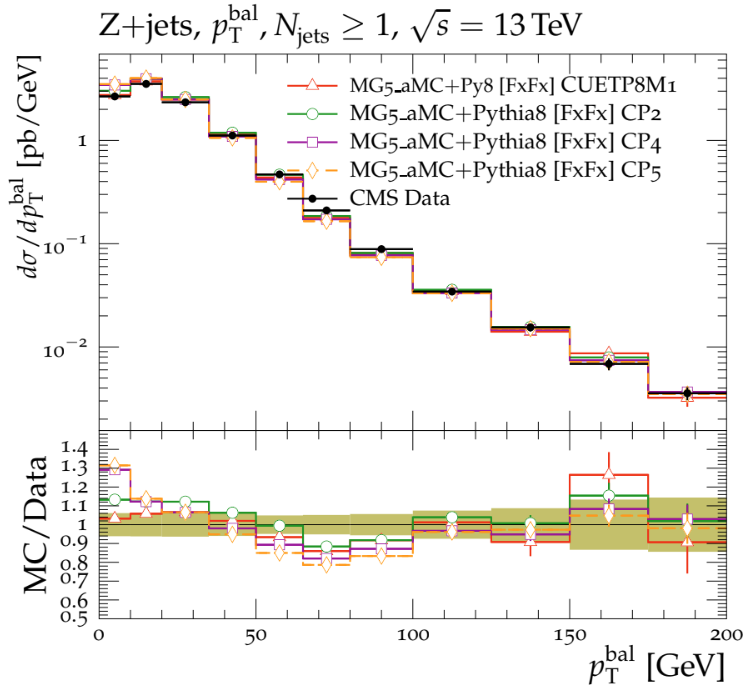
\includegraphics[width=0.985\textwidth]{{img/CPpaper_zjet1.png}}
	\end{subfigure}%
	\begin{subfigure}{0.5\textwidth}
		\centering
		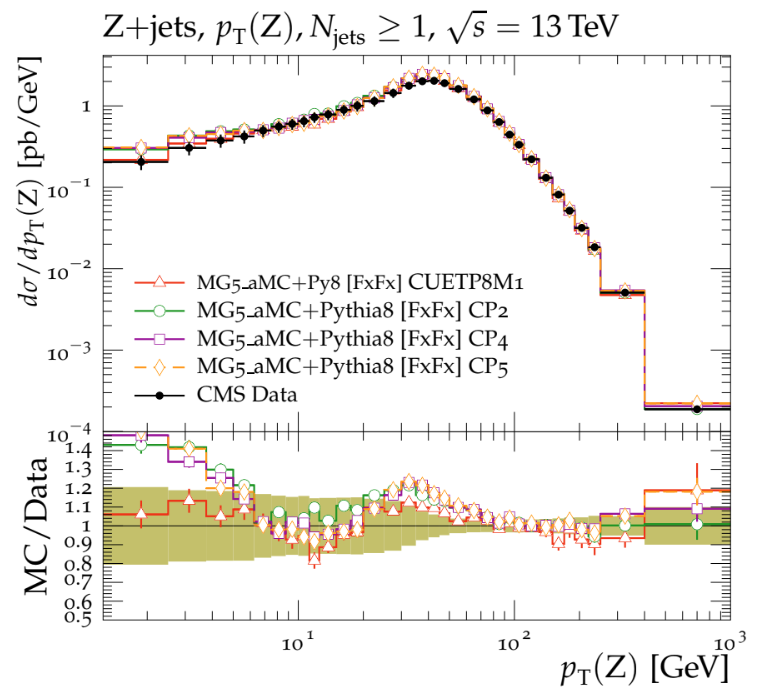
\includegraphics[width=\textwidth]{{img/CPpaper_zjet2.png}}
	\end{subfigure}%
	\caption{Figure taken from CP5 tune paper \cite{CPtunes}. These two images show the $Z$ boson production cross-section in $Z$ plus jets (with at least one jet) at $\sqrt{s}=13\ \mathrm{TeV}$ as a function of the imbalance of the transverse momentum between the jet and the $Z$ boson (left) and of the $Z$ boson transverse momentum (right) \cite{CMS:2018mdf}. The first bin in the left distribution and the region $p_T^Z \lesssim 40\ \mathrm{GeV}$, in the right one, is not well described by the CP5 tune (yellow line).}
	\label{fig:CP5_notdescribeZjet}
\end{figure}

\begin{figure}[!htb]
	\centering
	\noindent
	\begin{subfigure}{0.5\textwidth}
		\centering
		\includegraphics[width=\textwidth]{{img/rivet-plots-PrimordialkT_only_CP5default/CMS_2019_I1753680/d27-x01-y03.pdf}}
	\end{subfigure}%
	\begin{subfigure}{0.5\textwidth}
		\centering
		\includegraphics[width=\textwidth]{{img/rivet-plots-PrimordialkT_only_CP5default/CMS_2019_I1753680/d28-x01-y03.pdf}}
	\end{subfigure}
	\caption{The CP5 tune (red line) compared to the $Z$ boson production cross-section as a function of the $Z$ boson transverse momentum (left) or of the $\phi_\eta^*$ angle. This distributions showed here are from the CMS analysis \cite{ZpT_distributions} at the center-of-mass energy of $13\ \mathrm{TeV}$. The high region of the spectrum is not well described because it has been simulated only event to the LO, while a good description of it requires higher order matrix calculations.}
	\label{fig:CP5_notdescribeZ}
\end{figure}

\section{Primordial $k_T$ and ISR effect on $p_T^Z$}

The parameters that have been investigated in order to tune data and explain the $Z$ boson $p_T$ spectrum are:
\begin{itemize}
\item \texttt{BeamRemnants:primordialKThard} that set the width of the Gaussian distribution for the primordial $k_T$ sampling;
\item \texttt{SpaceShower:pT0Ref} that sets the threshold for the initial state radiation to take place.
\end{itemize}
Now, it is discussed how this parameter impact the $Z$ boson production transverse momentum spectrum. If only the LO diagram for the $Z$ production (\figRef{fig:feynamn_primkT_Zboson}a) is considered, one can only have a $Z$ production with zero transverse momentum. So the $Z$ boson $p_T^Z$ spectrum expected at LO is a $\delta$-distribution function centered on zero.  

\begin{figure}[!htb]
	\centering
	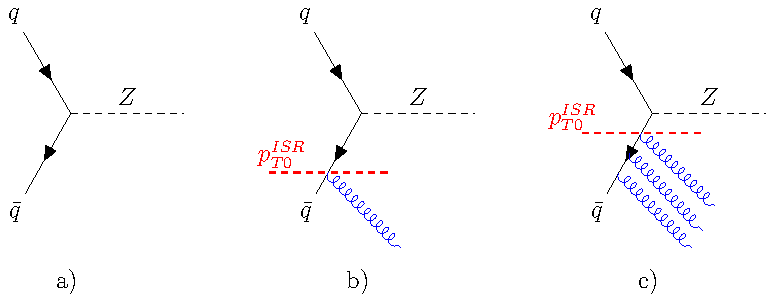
\includegraphics[width=0.8\textwidth]{{img/feynman_ZpT_2_blue.pdf}}
	\caption{$Z$ boson production diagrams: a) shows the LO diagram; b) is the LO diagram whit a high threshold for the ISR so it is produced a small amount of it; c) is the same but with a lower threshold for the ISR and a larger amount, in b) and c) cases the $Z$ boson can be produced with a non-zero transverse momentum, balanced by the ISR.}
	\label{fig:feynamn_primkT_Zboson}
\end{figure}

\noindent With the addition of the primordial $k_T$ a Gaussian distribution is obtained, whose width is set by \texttt{BeamRemnants:primordialKThard}.
If one moves to higher-order diagrams the $Z$ boson can be produced with a non zero $p_T$ that is balanced by the various jets, then the primordial $k_T$ is added to the already non-zero $Z$ boson transverse momentum. 
\\
The $Z$ boson can be produced with a non-zero trasverse momentum, balanced by the amount of ISR that is emitted from the incoming partons, in fact, each split can give to the incoming parton a non-zero initial value of $p_T$ and so the $Z$ boson is created with a non-zero $p_T$ before the introduction of the primordial $k_T$. 
\\
%A higher amount of ISR, so a lower value for the threshold, can lead to a larger $p_T$ taken from the parton that then can generate the $Z$ boson with a higher $p_T$ and vice versa.

\section{Primordial $k_T$ tune}

%The primordial $k_T$ was not investigated by CP5 so it is important to include that in the analysis in order to describe better the low $p_T$ region. 

The parameters variation ranges used for the tune are the ones reported in the \tableRef{table:primordialkT_variations} while other parameters are set to CP5 values.



\begin{table}[!htb]
\centering
\begin{tabular}{l | c }
Parameter Name & Value \\ 
\hline \hline
\\[-0.85em]
	\texttt{BeamRemnants:primordialKThard} & $[0.5 - 5.0]$\\[2pt]
	\texttt{SpaceShower:pT0Ref} & $[0.5 - 5.0]$\\
\end{tabular}
\caption{Variation ranges for the sampling used in the primordial $k_T$ tune.}
\label{table:primordialkT_variations}
\end{table} 

The number of samples is lower than the one used for the Underlying Event. The training set that has been used for the PerBin Model contains $160$ MC runs and $200$ for the Inverse Model, this is related to the lower number of parameters to tune. So, the operation of the tune was computationally faster: less Monte Carlo jobs to run.
\\
\figRef{fig:CP5_notdescribeZ} shows the distributions used to perform the tune. The distributions  are from the \cite{ZpT_distributions} analysis at $\sqrt{s}=13\ \mathrm{TeV}$:
\begin{itemize}
	\item The $Z$ boson production cross-section in Drell Yan measurements as a function of $p_T^Z$;
	\item The $Z$ boson production cross-section in Drell Yan measurements as a function of $\phi_\eta^*$.
\end{itemize}

\noindent Note that the region of interest is the low $p_T$ region. The simulation of the whole spectrum requires the adoption of a merging scheme between the higher-order matrix element calculations and parton shower, as FxFx, which is computationally expensive. The strategy followed was the tuning of the low region, the one of interest, taking only the first five bins from each distribution.  


\medskip

\noindent The PerBin Model minimization results are displayed in \figRef{fig:result_PerBin_PrimordialkT_1}. The blue line indicates the value of the $\chi^2/DoF$ as a function of the parameter value. The best estimation is marked by a solid red line while the dashed red lines indicate the errors, these results are reported in \tableRef{table:Primordial_kT_results}. Both the parameters are in a well-defined minimum so the minimization phase work properly. 

\begin{figure}[!htb]
	\centering
	\noindent 
	\begin{subfigure}{0.48\textwidth}
	\centering
		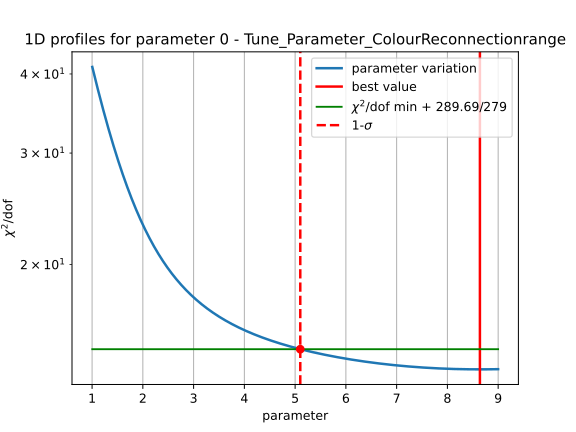
\includegraphics[width=\textwidth]{{img/chi2_0.png}}
	\end{subfigure}%
	\begin{subfigure}{0.48\textwidth}
	\centering
		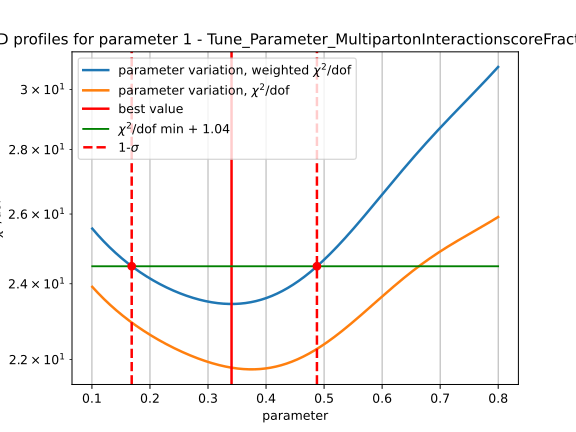
\includegraphics[width=\textwidth]{{img/chi2_1.png}}
	\end{subfigure}
	\caption{The output of the minimizer for the PerBin model in the primordial $k_T$ tune. The left panel shows the result of the minimization for the \texttt{SpaceShower:pT0Ref} parameter while the right one \texttt{BeamRemnants:primordialKThard}. The blue line is the $\chi^2/\mathrm{DoF}$ the best value is indicated by the solid red line while the errors are the ones indicated by the dashed red lines.}
	\label{fig:result_PerBin_PrimordialkT_1}
\end{figure}

\medskip

The Inverse model distribution of predictions for the best model is reported in \figRef{fig:PrimordialkT_InverseModel_results}: the best estimation for the parameter is indicated by the solid black line while the dashed black lines are the errors computed using the standard deviation. The hyperparameter space scanned to search for these best model is the same used above and reported in \tableRef{table:hyperpar_MinBias_2par}. At the end of the scanning, the best hyperparameters obtained are the ones reported in the \tableRef{table:hyperpar_PrimkT}.


\begin{figure}[!htb]
	\centering
	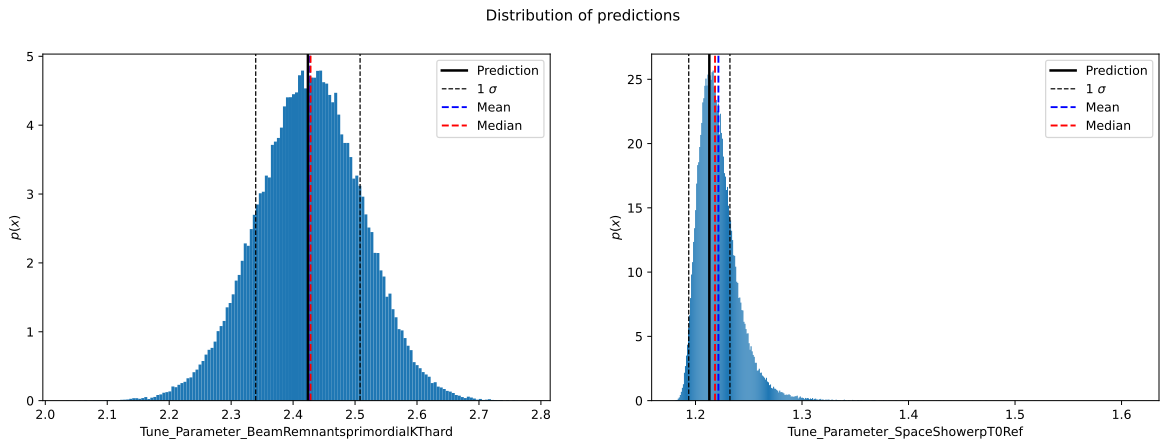
\includegraphics[width=0.95\textwidth]{{img/prediction_spread.png}}
	\caption{The prediction spread for the Inverse model in the primordial $k_T$ tune. The left histogram refers to the \texttt{BeamRemnants:primordialKThard} parameter while the right one to the \texttt{SpaceShower:pT0Ref}. The predictions are indicated by the solid black vertical lines and the errors by the dashed black lines. }
	\label{fig:PrimordialkT_InverseModel_results}
\end{figure}

\begin{table}[!htb]
	\centering
	\begin{tabular}{ l | c }
	Hyperparameter & Value\\[2pt]\hline\hline
	Number of hidden layers & 2 \\[2pt]
	Units layers & [15,\,17] \\[2pt]
	Activation function & sigmoid \\[2pt]
	Optimizer & rmsprop\\[2pt]
	Epochs & 2000\\[2pt]
	Batch size & 64\\[2pt]
	\end{tabular}
	\caption{Best hyperparameters model found for the primordial $k_T$ tune with Inverse model.}
	\label{table:hyperpar_PrimkT}
\end{table}


\noindent The PerBin Model values and errors obtained as output from the tune are reported in \tableRef{table:Primordial_kT_results}.  
These are also compared to the ones obtained from the Inverse model. The value obtained from the two \textsc{mcnntunes} models are compatible with each other. The default values for CP5 are also reported and they are the ones inherited by the Monash tune \cite{Monash}. The values obtained by the tunes based on \textsc{mcnntunes} are quite different to the ones in CP5.  

\begin{table}
	\centering
\begin{tabular}{l | c | c | c}
Parameter Name & PerBin & Inverse & Default CP5\\ 
\hline \hline
\\[-0.85em]
	\texttt{BeamRemnants:primordialKThard} & $ 2.5^{+0.2}_{-0.2} $ & $ 2.42\pm0.08 $ & $1.8$\\
	\texttt{SpaceShower:pT0Ref} & $ 1.6^{+0.5}_{-0.5} $ & $ 1.21\pm0.02  $ & $2.0$
\end{tabular}
\caption{Results obtained from the PerBin and the Inverse model in the tuning of the low region of $Z$ boson production spectra. They are compared to the default for CP5 (inherited from Monash tune.)}
\label{table:Primordial_kT_results}
\end{table}	

\medskip

The overall results are displayed in \figRef{fig:result_primKT_FXFX}. These new tunes describe better the low regions of the two spectra. These low regions are the ones  actually tuned, the higher $p_T$ region is only simulated using the value obtained from the tune of the first 5 bins in each distribution of \figRef{fig:result_primKT_FXFX}. To simulate all the spectrum it has been employed the FxFx margin scheme in order to avoid double-counting and get a correct result from the simulation.

 

 
%\begin{figure}[!htb]
%	\centering
%	\noindent
%	\begin{subfigure}{0.48\textwidth}
%	\centering
%	\includegraphics[width=\textwidth]{{img/rivet-plots-PrimordialkT_PerBin_vs_Inverse_vs_CP5_FxFx_weights/CMS_2019_I1753680/d27-x01-y03.pdf}}	
%	\end{subfigure}%
%	\begin{subfigure}{0.48\textwidth}
%	\centering
%	\includegraphics[width=\textwidth]{{img/rivet-plots-PrimordialkT_PerBin_vs_Inverse_vs_CP5_FxFx_weights/CMS_2019_I1753680/d28-x01-y03.pdf}}	
%	\end{subfigure}
%	\label{fig:result_primKT_FXFX}
%\end{figure}



%\begin{figure}[!htb]
%	\centering
%	\noindent
%	\begin{subfigure}{0.48\textwidth}
%	\centering
%	\includegraphics[width=\textwidth]{{img/rivet-plots-PrimordialkT_PerBin_vs_Inverse_vs_CP5_FxFx_noWeights/CMS_2019_I1753680/d27-x01-y03.pdf}}	
%	\end{subfigure}%
%	\begin{subfigure}{0.48\textwidth}
%	\centering
%	\includegraphics[width=\textwidth]{{img/rivet-plots-PrimordialkT_PerBin_vs_Inverse_vs_CP5_FxFx_noWeights/CMS_2019_I1753680/d28-x01-y03.pdf}}	
%	\end{subfigure}
%	\caption{The results we get from the tune of the primordial $k_T$. The left figure shows the $Z$ boson production cross-section as a function of the $p_T^Z$.  
%The red line refers to the PerBin model tune, the blue line to the Inverse Model and the green line is the CP5 default tune. The black points are the experimental data. The colored vertical lines the statistical uncertainties.
%	It is clear that our two tunes better describe the low region with respect to the original CP5. }
%	\label{fig:result_primKT_FXFX}
%\end{figure}
\begin{figure}[!htb]
	\centering
	\noindent
	\begin{subfigure}{0.48\textwidth}
	\centering
	\includegraphics[width=\textwidth]{{img/rivet-plots-PrimordialkT_PerBin_vs_Inverse_vs_CP5_FxFx_ext_ext_noWeights_Final/CMS_2019_I1753680/d27-x01-y03.pdf}}	
	\end{subfigure}%
	\begin{subfigure}{0.48\textwidth}
	\centering
	\includegraphics[width=\textwidth]{{img/rivet-plots-PrimordialkT_PerBin_vs_Inverse_vs_CP5_FxFx_ext_ext_noWeights_Final/CMS_2019_I1753680/d28-x01-y03.pdf}}	
	\end{subfigure}
	\caption{The results obtained from the tune of the primordial $k_T$. The left figure shows the $Z$ boson production cross-section as a function of the $p_T^Z$.  
The red line refers to the PerBin model tune, the blue line to the Inverse Model and the green line is the CP5 default tune. The black points are the experimental data. The colored vertical lines the statistical uncertainties.
	It is clear that the two tunes based on \textsc{mcnntunes} better describe the low region with respect to the original CP5. }
	\label{fig:result_primKT_FXFX}
\end{figure}


\section{Primordial $k_T$ tune vs MPI}

As discussed above primordial $k_T$ is not the only source of non zero transverse momentum in LO $Z$ boson production.
This is the reason why also the parameter that controls the amount of Initial State Radiation is tuned here. As described above, the ISR can leads to a non zero initial transverse momentum a larger amount of ISR (low \texttt{SpaceShower:pT0Ref}) is related to more splitting occurring in the evolution of the incoming partons before these partons undergo the hard scattering in which the $Z$ boson is produced. But this is not the only process that can lead to a non-zero initial transverse momentum, there are also the MPI that can contribute to this initial transverse momentum. It is not an easy task to understand the effect of MPI on the $p_T$ of the produced $Z$ boson. 

\figRef{fig:result_primKT_MPI1} shows the effect of the MPI on the distributions used for the tune. The blue line is obtained setting \texttt{PartonLevel:MPI=off} in \textsc{Phytia8} configuration. It has been performed a calculation employing only a LO calculation, so the FxFx margin scheme is not required for this simulation. The high region of the distribution is not well described by the LO calculation but in this case the effect of the MPI are expected only in the low-$p_T^Z$ region.

\begin{figure}[!htb]
	\centering
	\noindent
	\begin{subfigure}{0.48\textwidth}
	\centering
	\includegraphics[width=\textwidth]{{img/rivet-plots-PrimordialkT_with_without_MPI_yellowBand/CMS_2019_I1753680/d27-x01-y03.pdf}}	
	\end{subfigure}%
	\begin{subfigure}{0.48\textwidth}
	\centering
	\includegraphics[width=\textwidth]{{img/rivet-plots-PrimordialkT_with_without_MPI_yellowBand/CMS_2019_I1753680/d28-x01-y03.pdf}}	
	\end{subfigure}
	\caption{The image shows that MPI have an effect on the two distribution. The blue line is the result without the MPI  (\texttt{PartonLevel:MPI=off}) and the red line with MPI. FxFx has not been used here: the high regions of the spectra are not well  described by the simulation.}
	\label{fig:result_primKT_MPI1}
\end{figure}

The main parameter that controls the number of parton interactions in a single hadron-hadron collision is the \texttt{MultipartonInteractions:}\-\texttt{pT0Ref} parameter. It is clear that the first $2$ or $3$ bins of the left distribution of \figRef{fig:result_primKT_MPI1_pt0} are sensitive to the variation of this parameter. A future thing to do is to investigate the effects of these MPI in more detail and perform a more general tune including them in this description.


\begin{figure}[!htb]
	\centering
	\noindent
	\begin{subfigure}{0.48\textwidth}
	\centering
	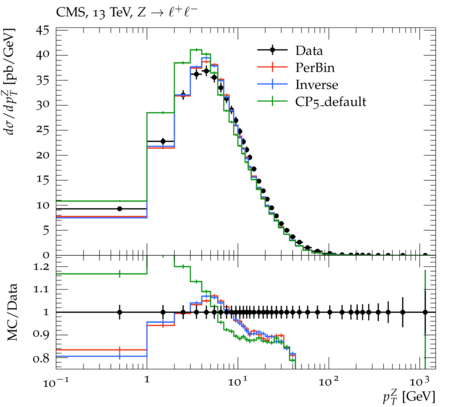
\includegraphics[width=\textwidth]{{img/rivet-plots-primordialkT_vs_MPI_finale/d27-x01-y03.png}}	
	\end{subfigure}%
	\begin{subfigure}{0.48\textwidth}
	\centering
	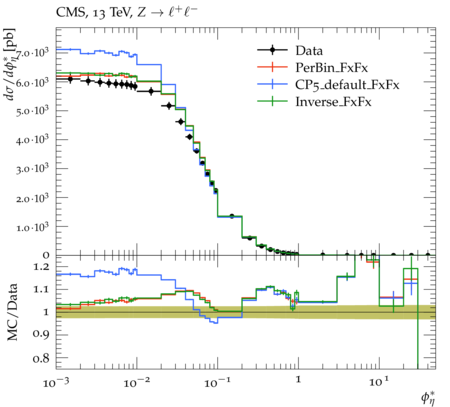
\includegraphics[width=\textwidth]{{img/rivet-plots-primordialkT_vs_MPI_finale/d28-x01-y03.png}}	
	\end{subfigure}
	\caption{The image shows that \texttt{MPI:pT0Ref} affect the first bins of the left distribution. The black points are the experimental data while the various colored lines are the simulations with different values for the parameter that controls the \texttt{MPI:pT0Ref}. FxFx has not been used here: the high regions of the spectra are not well  described by the simulation.}
	\label{fig:result_primKT_MPI1_pt0}
\end{figure}


